% !TEX TS-program = pdflatex
% !TEX encoding = UTF-8 Unicode

% This is a simple template for a LaTeX document using the "article" class.
% See "book", "report", "letter" for other types of document.

\documentclass[10pt,twocolumn]{article}

\usepackage[utf8]{inputenc} % set input encoding (not needed with XeLaTeX)
\usepackage{graphicx}
\usepackage{listings} 
\usepackage{xcolor,colortbl}
\usepackage[section]{placeins}
\usepackage{amsthm}
\usepackage{amssymb}
\usepackage{amsthm}
\usepackage{mathtools}
\graphicspath{ {images/} }

%%% Examples of Article customizations
% These packages are optional, depending whether you want the features they provide.
% See the LaTeX Companion or other references for full information.

%%% PAGE DIMENSIONS
\usepackage{geometry} % to change the page dimensions
\geometry{a4paper} % or letterpaper (US) or a5paper or....
\geometry{margin=0.55in} % for example, change the margins to 2 inches all round
% \geometry{landscape} % set up the page for landscape
%   read geometry.pdf for detailed page layout information

\usepackage{graphicx} % support the \includegraphics command and options

% \usepackage[parfill]{parskip} % Activate to begin paragraphs with an empty line rather than an indent

%%% PACKAGES
\usepackage{booktabs} % for much better looking tables
\usepackage{array} % for better arrays (eg matrices) in maths
\usepackage{paralist} % very flexible & customisable lists (eg. enumerate/itemize, etc.)
\usepackage{verbatim} % adds environment for commenting out blocks of text & for better verbatim
\usepackage{subfig} % make it possible to include more than one captioned figure/table in a single float
\usepackage{indentfirst}
% These packages are all incorporated in the memoir class to one degree or another...

%%% HEADERS & FOOTERS
\usepackage{fancyhdr} % This should be set AFTER setting up the page geometry
\pagestyle{fancy} % options: empty , plain , fancy
\renewcommand{\headrulewidth}{0pt} % customise the layout...
\lhead{}\chead{}\rhead{}
\lfoot{}\cfoot{\thepage}\rfoot{}

%%% SECTION TITLE APPEARANCE
\usepackage{sectsty}
\allsectionsfont{\sffamily\mdseries\upshape} % (See the fntguide.pdf for font help)
% (This matches ConTeXt defaults)

%%% ToC (table of contents) APPEARANCE
\usepackage[nottoc,notlof,notlot]{tocbibind} % Put the bibliography in the ToC
\usepackage[titles,subfigure]{tocloft} % Alter the style of the Table of Contents
\renewcommand{\cftsecfont}{\rmfamily\mdseries\upshape}
\renewcommand{\cftsecpagefont}{\rmfamily\mdseries\upshape} % No bold!
\setlength{\parindent}{0.5cm} 

%%% END Article customizations

%%% The "real" document content comes below...

\title{On Fast Search of First Confirmation Of Goldbach's Strong Conjecture}
\author{Marcin Barylski}
\date{\small{Published: May 8, 2016 \\ The last update: December 29, 2019}}

\definecolor{Gray}{gray}{0.85}
\definecolor{LightCyan}{rgb}{0.88,1,1}
\newcolumntype{a}{>{\columncolor{Gray}}c}
\newcolumntype{b}{>{\columncolor{white}}c}

\newtheorem{theorem}{Theorem}
\newtheorem{lemma}[theorem]{Lemma}

\newcommand\bigforall{\mbox{\huge $\mathsurround5pt\forall$}} 
\newcommand\bigexists{\mbox{\huge $\mathsurround5pt\exists$}} 

\begin{document}
\maketitle

\begin{abstract}
Goldbach strong conjecture states that all even integers $n \textgreater 2$ can be expressed as the sum of two prime numbers (Goldbach partitions of $n$). Hypothesis still remains open and is confirmed experimentally for bigger and bigger $n$. This work studies different approaches to finding the first confirmation of this conjecture in order to select the most effective confirmation method.
\end{abstract}

\section{Introduction}

Goldbach strong (also called binary) conjecture asserts that all positive even integer $n$ $\geq$ 4 can be expressed as the sum of two prime numbers. This hypothesis, formulated by Goldbach in 1742 in letter to Euler \cite{goldbach1742} and then updated by Euler to the form above is one of the oldest and still unsolved problems in number theory. Empirical verification showed that it is true for all $n$ $\leq$ 4 x $10^{18}$ \cite{oliveira2012}.\par
The expression of a given number $n$ as a sum of two primes $p_1$ and $p_2$ is called a Goldbach Partition (GP) of $n$. Let's denote this relation as $GSC(n, p_1, p_2)$. Then Goldbach strong conjecture can be written as (1):

\begin{equation}
\displaystyle\mathop{\bigforall}_{x \textgreater 1, x \in \mathbb{N}} \displaystyle\mathop{\bigexists}_{p_1, p_2 \in \mathbb{P}} GSC (2x, p_1, p_2)
\end{equation}

\begin{figure}[!ht]
\centering
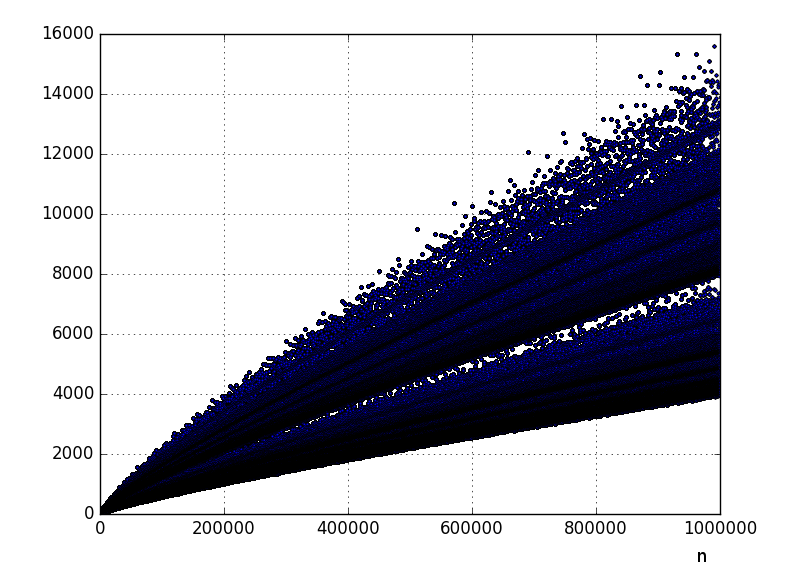
\includegraphics[width=9cm]{f_pairs}
\caption{$r(n)$ ($2$ \textless $n$ \textless $10^6$, $n = 2k, k \in \mathbb{N}$)}
\label{fig:pairs}
\end{figure}

Let $r(n)$ be the number of GPs of $n$ and let $R(n)$ be a set of distincs GPs of $n$ (uniqueness guaranteed through $p_1$  $\leq$ $p_2$). Goldbach strong conjecture may be rewritten that $r(n) > 0$ for all positive even integers $n$ $\geq$ 4. Computational experiments show (for $n$ \textless $10^6$) that the hyphothesis may be reinforced: bottom estimation for $min(r(n))$ is increasing with $n$ (Figure $\ref{fig:pairs}$). \cite{woon2000} formulates conjecture that lower and upper bounds can be expressed as simple exponentials.\par

Empirical verification of Goldbach strong conjecture and search for GP requires fast and reliable primality test, repeated even twice for both components of a candidate for GP. The following paper is devoted to designing of the fastest algorithm for searching the first confirmation: a pair of primes: $p_1$  and $p_2$ for $n$, where $GSC (n, p_1, p_2)$. Design of algorithm is based on detailed observations for all GPs found for all even $n$ (4 $\leq$ $n$ \textless $10^6$), and then confirmed for bigger numbers. All listings are written in Python programming language and published at \cite{github}. \par

\section{Fast primality test}

For the sake of this work, to check if a given number is prime or not, algorithm skewed in Listing 1 was used. Presented approach is taking advantage of preloaded prime and composite sets (containing prime and composite numbers found earlier) which gives instant result. Then, algorithm is testing if a candidate for prime is even (divides it by $2$) or is a multiple of $3$ - in case of success the candidate is confirmed as a composite number. Eventually, it is taking advantage of Lemma 1.

\lstset{language=Python}
\lstset{breaklines=true}
\lstset{frame=shadowbox}
\lstset{caption={Primality test}}
\begin{lstlisting}[linewidth=8.7cm]
# input: integer n
# external dependencies:
#   prime_set - a set of primes
#   composite_set - a set of non-primes
# output: True if n is prime; False otherwise
def  is_prime (n):
  if n<=1:
    return False
  elsif n<=3:
    return True
  elsif n in prime_set:
    return True
  elsif n in composite_set:
    return False
  elsif n%2 == 0 or n%3 == 0:
    return False
  i=5
  while i*i<=n:
    if n%i == 0 or n%(i+2) == 0:
      return False
     i+=6
  return True
\end{lstlisting}

\begin{lemma}
Every prime $p \textgreater 3$ can be written as $p=6k \pm 1$ (where $k$ is a positive integer).
\end{lemma}
\begin{proof}
Every positive integer $n$ $\geq$ 6 can be expressed as $6k+m$, where $m$=0, 1, \ldots, 5, $k$ $\geq$1. Numbers $6k$, $6k+2$, $6k+3$ and $6k+4$ are always composite because they are divisible by either $2$ or $3$ or both ($6k$=$2\times 3k$, $6k$+2=2$\times (3k+1)$, $6k+3$=$3\times (2k+1)$, $6k+4$=$2 \times (3k+2))$. $6k+1$ and $6k+5$ are either prime (ie. $6 \times 1+1=7$, $6 \times 2-1=11$) or composite (ie. $6k+5$ is divisible by $5$ if $k$ is multiple of $5$, $6k+1$ is divisible by $3$ if sum of decimal digits is divisible by $3$). $6k+5$ can be rewritten as $6 \times (k+1)-1$. All primes \textless $5$ ($2$ and $3$) cannot be expressed as $p=6k \pm 1$ where $k$ is a positive integer. This means that every prime $p$ $\geq$ $5$ can be expressed as $6k \pm 1$ (where $k \geq 1$).
\end{proof}

\section{Characteristics of GPs}

The first part of work is devoted to detailed examination of different characteristics of $R(n)$ ($n$ \textless $10^6$) in order to find useful observations which are the foundation of further versions of GP fast confirmation algorithms.

\subsection{Difference between primes in GP}

First analysis concentrates on possible differences between primes in $R(n)$ (for $n$ \textless $10^6$), including the smallest, average and the biggest difference. \par
Tests show that minimal difference may be low (comparing to $n$). In majority of examined cases it is below 1000, with just  six recorded examples above 2000 (Figure $\ref{fig:mindiff}$). The bold observation may lead to a hypothesis that primes in at least one GP in $R(n)$ are not so far from each other (2): \par

\begin{equation}
\displaystyle\mathop{\bigforall}_{k \textgreater 1, k \in \mathbb{N}} \displaystyle\mathop{\bigexists}_{GSC (2k, p_1, p_2)}\displaystyle\mathop{\bigexists}_{C \in \mathbb{N}} C = \mid p_1 - p_2 \mid \ll 2k
\end{equation}

\begin{figure}[ht]
\centering
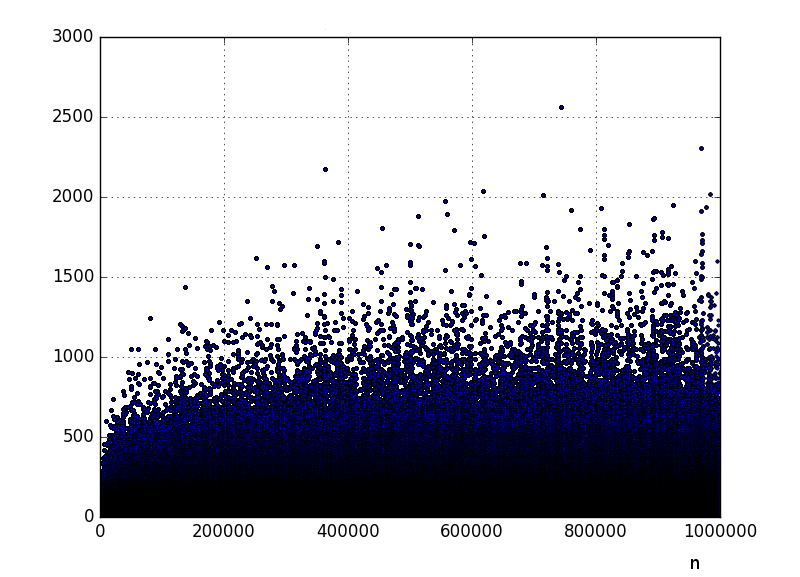
\includegraphics[width=9cm]{f_min_diff_pairs}
\caption{Minimal difference in $R(n)$ ($2$ \textless $n$ \textless $10^6$)}
\label{fig:mindiff}
\end{figure}

Maximum difference in GP is close to $n$, indicating that $p_2$ in such extreme case ($p_1$ $\leq$  $p_2$) is close to $n$ (Figure $\ref{fig:maxdiff}$). Average difference in GP is fluctuating slightly above $\frac{n}{2}$ (Figure $\ref{fig:avgdiff}$). The bigger $n$, the more visible fluctuations. \par

\begin{figure}[ht]
\centering
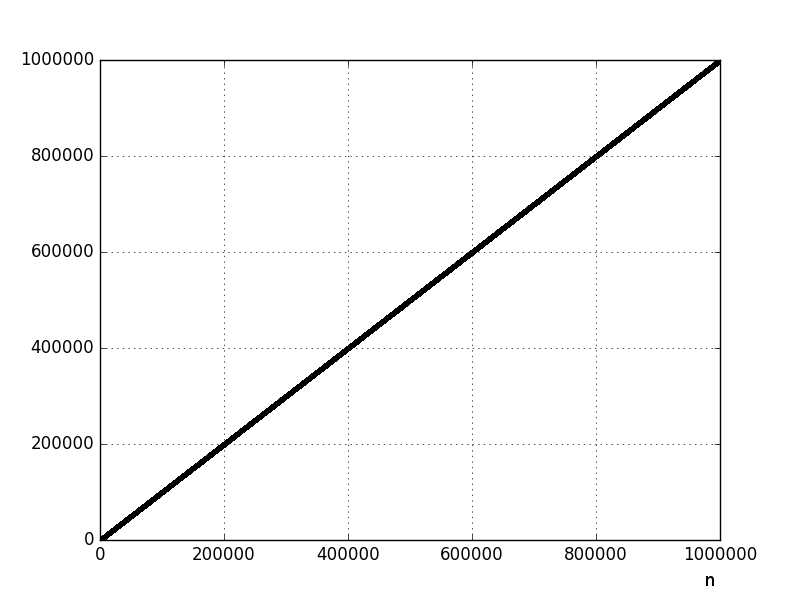
\includegraphics[width=9cm]{f_max_diff_pairs}
\caption{Maximum difference in $R(n)$ ($2$ \textless $n$ \textless $10^6$)}
\label{fig:maxdiff}
\end{figure}

\begin{figure}[ht]
\centering
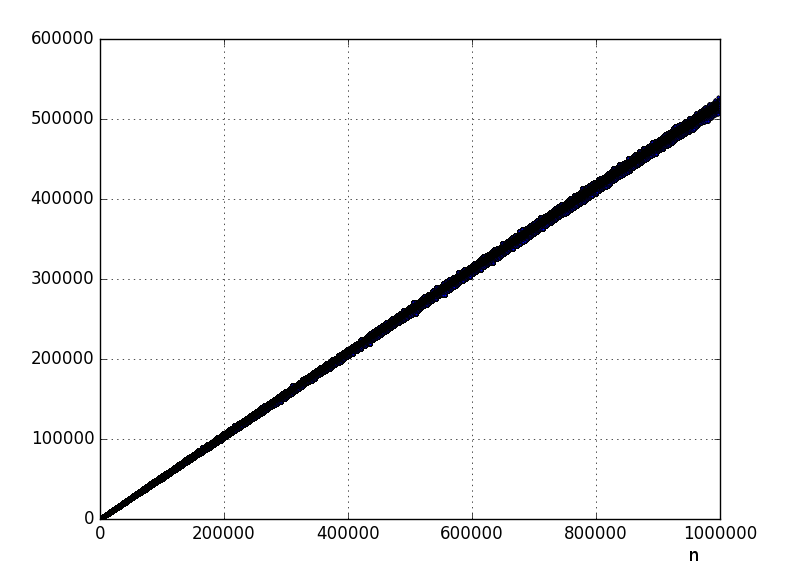
\includegraphics[width=9cm]{f_avg_diff_pairs}
\caption{Average difference in $R(n)$ ($2$ \textless $n$ \textless $10^6$)}
\label{fig:avgdiff}
\end{figure}

Further observation of trends in change of minimum / maximum / average difference in GPs of $n$ (+1 if difference between previous and current value is positive, -1 if negative, +0 if no change) shows that all those three trends are generally descending, with just few ascending episodes (Figure $\ref{fig:trends2000}$). Big picture (Figure $\ref{fig:trends}$) presents that both trends for minimum and average difference have very similar characteristics. 

\begin{figure}[ht]
\centering
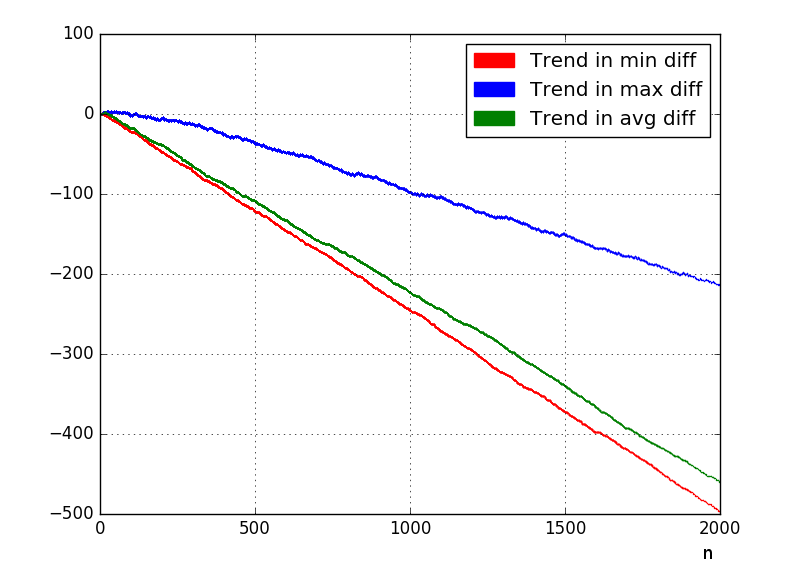
\includegraphics[width=9cm]{f_trends_2000_pairs}
\caption{Trends in $R(n)$ for the smallest $n$ ($2$ \textless $n$ \textless $2000$)}
\label{fig:trends2000}
\end{figure}

\begin{figure}[!ht]
\centering
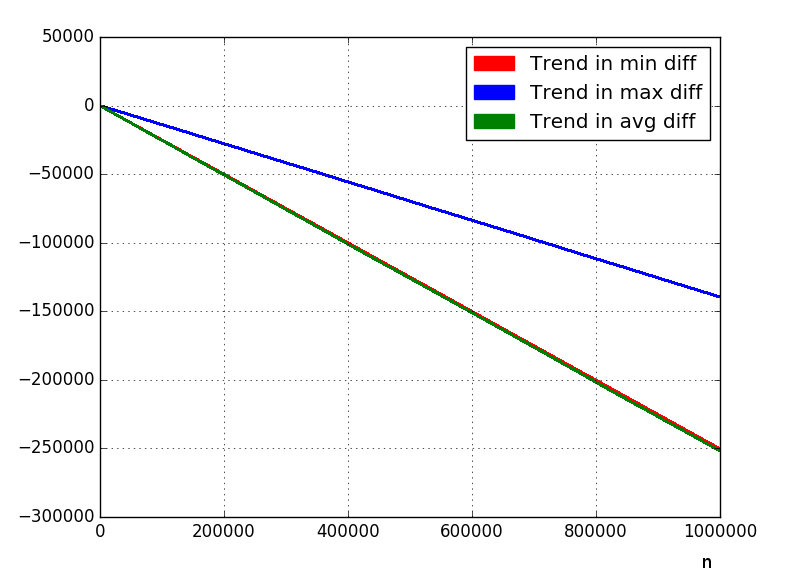
\includegraphics[width=9cm]{f_trends_pairs}
\caption{Trends in $R(n)$ ($2$ \textless $n$ \textless $10^6$)}
\label{fig:trends}
\end{figure}

\subsection{Minimal prime in GP}

Detailed examination of $R(n)$ ($n$ \textless $10^6$) shows that the minimal prime in at least one of GPs is usually low (Figure $\ref{fig:minprime}$). For all $n$ \textless $10^6$  it has been computionally verified that 523 is the biggest minimal prime (for $n$=503222) in all possible GPs. \cite{oliveira2012} verified that 3325581707333960528 is the smallest number that has no GP with a prime below 9781. Among the smallest primes in GBs ($n$ \textless $10^6$) the most popular is 3 (Table $\ref{tablesmallprimes}$). \par

\begin{figure}[!ht]
\centering
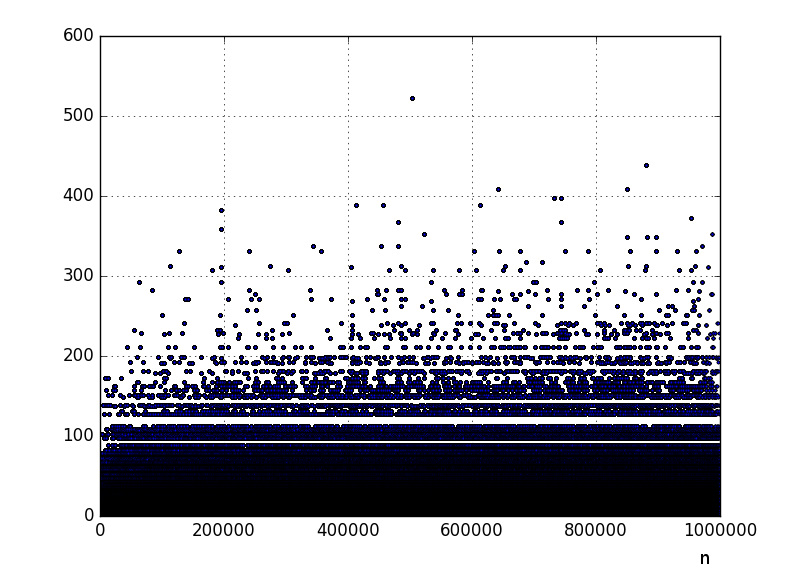
\includegraphics[width=9cm]{f_min_prime_in_sum}
\caption{Minimal prime in $R(n)$ ($2$ \textless $n$ \textless $10^6$)}
\label{fig:minprime}
\end{figure}

\begin{table}[!ht]
\centering
\caption{Smallest primes in $R(n)$ ($2$ \textless $n$ \textless $10^6$)}
\label{tablesmallprimes}
\begin{tabular}{|a|b|a|b|}
  \hline 
  \rowcolor{LightCyan}
  Prime & Appearances & Prime & Appearances \\
  \hline
2 & 1 & 79 & 101 \\
  \hline
3 & 78497 & 181 & 219 \\
  \hline
5 & 70328 & 191 & 76 \\
  \hline
7 & 62185 & 193 & 109 \\
  \hline
11 & 48582 & 197 & 49 \\
  \hline
13 & 40916 & 199 & 112 \\
  \hline
17 & 31091 & 211 & 97 \\
  \hline
19 & 29791 & 223 & 40 \\
  \hline
23 & 21422 & 227 & 37 \\
  \hline
29 & 16776 & 229 & 42 \\
  \hline
31 & 18119 & 233 & 32 \\
  \hline
37 & 13165 & 239 & 25 \\
  \hline
41 & 10001 & 241 & 41 \\
  \hline
43 & 9100 & 251 & 19 \\
  \hline
47 & 6625 & 257 & 12 \\
  \hline
53 & 5076 & 263 & 9 \\
  \hline
59 & 4012 & 269 & 3 \\
  \hline
61 & 6417 & 271 & 22 \\
  \hline
67 & 4839 & 277 & 15 \\
  \hline
71 & 2597 & 281 & 4 \\
  \hline
73 & 2801 & 283 & 17 \\
  \hline
79 & 3030 & 293 & 8 \\
  \hline
83 & 1753 & 307 & 14 \\
  \hline
89 & 1442 & 311 & 3 \\
  \hline
97 & 1763 & 313 & 7 \\
  \hline
101 & 988 & 317 & 2 \\
  \hline
103 & 1266 & 331 & 12 \\
  \hline
107 & 889 & 337 & 4 \\
  \hline
109 & 1245 & 349 & 3 \\
  \hline
113 & 507 & 353 & 2 \\
  \hline
127 & 730 & 359 & 1 \\
  \hline
131 & 356 & 367 & 2 \\
  \hline
137 & 358 & 373 & 1 \\
  \hline
139 & 602 & 383 & 1 \\
  \hline
149 & 279 & 389 & 3 \\
  \hline
151 & 522 & 397 & 2 \\
  \hline
157 & 253 & 409 & 2 \\
  \hline
163 & 258 & 439 & 1 \\
  \hline
167 & 168 & 523 & 1 \\
  \hline
\end{tabular} 
\end{table}

\subsection{Twin primes in GP}

\cite{barylski2018} shows that original Goldbach conjecture could be extended to a form that every even $n \textgreater 4$ (this is (1) without case $n = 4 = 2 + 2$) can be expressed as a sum of twin prime and another prime (3):

\begin{equation}
\displaystyle\mathop{\bigforall}_{x \textgreater 2, x \in \mathbb{N}} \displaystyle\mathop{\bigexists}_{p_1 \in \mathbb{P_T}}  \displaystyle\mathop{\bigexists}_{p_2 \in \mathbb{P}}GSC (2x, p_1, p_2)
\end{equation}

Figure $\ref{fig:twinprimesall}$ depicts that number of distint twin primes in $R(n)$ is increasing with $n$.

\begin{figure}[!ht]
\centering
\captionsetup{justification=centering}
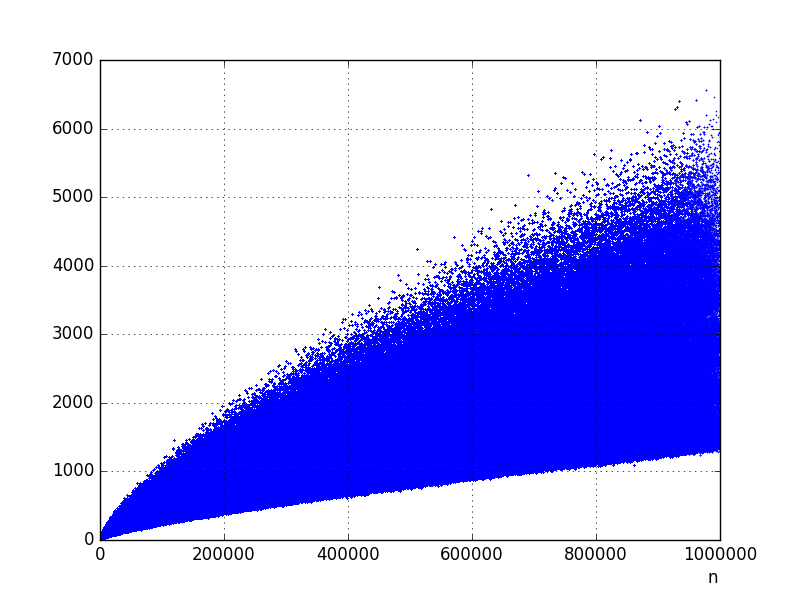
\includegraphics[width=9cm]{f_twin_primes_all}
\caption{Number of distinct twin primes in $R(n)$ \\ ($2$ \textless $n$ \textless $10^6$)}
\label{fig:twinprimesall}
\end{figure}

\subsection{GP and symmetrical primes}

We can rewrite Goldbach hypothesis to the following form: all positive integers \textgreater 1 can be expressed as a half of sum of two primes. This means that given integer $n$ \textgreater 1 is in fact a symmetry point for two primes $p_1$  and $p_2$. Let us call such $p_1$ and $p_2$ as symmetrical primes to $n$, denoting this symmetry as $psym(n,i) = (p_1,p_2)$, if there exists yet another integer $i$ ($0$ $\leq$ $i$ $\leq$ $n$ - $2$) that $p_1$ = $n$ - $i$ and $p_2$ = $n$ + $i$. For example, $2 = (2+2)/2$ ($psym(2,0)=(2,2)$), $3 = (3+3)/2$ ($psym(3,0)=(3,3)$), $4 = (3+5)/2$ ($psym(4,1)=(3,5)$). If $n$ is prime, then we always have $psym(n, 0)=(n,n)$. \par
Let $s(n)$ be a number of available symmetrical primes to $n$, and $S(n)$ a set of all symmetrical primes to $n$. Figure $\ref{fig:symprimes}$ which is depicting $s(n)$ has very similar shape to Figure $\ref{fig:pairs}$ which is depicting $r(n)$. Further empirical examination suggests that $s(n)$ and $r(n)$ are correlated what is depicted by Figure $\ref{fig:gptosymp}$. Each GP is built from two primes $p_1$ and $p_2$ which are symmetrical primes to $n$ = $\frac{p_1 + p_2}{2}$. $n$ is always a positive integer because every GP is built from either both odd primes or both even primes, thus sum of such two primes is always even. Each GP is constructed from two primes which are fulfilling $psym(\frac{p_1+p_2}{2}, \frac{p_2 - p_1}{2})$.\par

\begin{figure}[!ht]
\centering
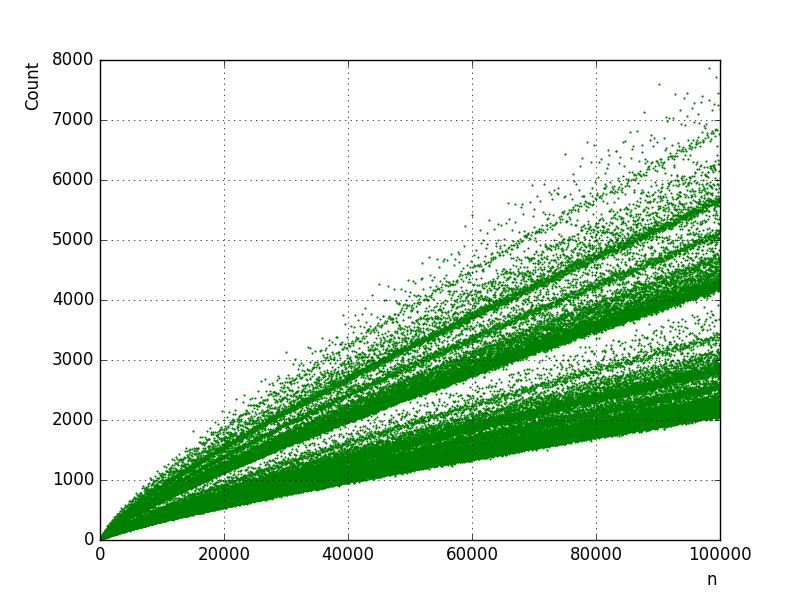
\includegraphics[width=9cm]{f_checkpoint_gap_num_of_sym_primes}
\caption{$s(n)$ ($2$ \textless $n$ \textless $10^5$)}
\label{fig:symprimes}
\end{figure}

\begin{lemma}
Every prime p \textgreater 3 can be written as $p=3x \pm 1$ (where $x$ is a positive integer).
\end{lemma}
\begin{proof}
All integers $n \textgreater 3$ can be written as $3x + i$, where $i = 0, 1, 2$ and $x \geq 1$. If $n_1 = 3x \textgreater 3$, then $n_1$ is always composite number, because $x \textgreater 1$ and both $3$ and $x$ divides $n_1$. On the other hand, numbers of form $3x-1$ can be either prime (ie. $5 = 3 \times 2 - 1$) or composite (ie. $8 = 3 \times 3 -1=2 \times 2 \times 2$) and numbers of form $3x+1$ can be either prime (ie. $7 = 3 \times 2 + 1$) or composite (ie. $10 = 3 \times 3 + 1=2 \times 5$).
\end{proof}

\begin{table}[ht]
\centering
\caption{Symmetrical primes to $n \textgreater 1$ ($a, x, k_1, k_2 \textgreater 0$)}
\label{tablesymprimes}
\begin{tabular}{|c|c|l|}
  \hline 
  \rowcolor{LightCyan}
  $n$ & $\frac{p_1+p_2}{2}$ & $(p_1, p_2)$ \\
  \hline 
  2 & $3 \times 1 - 1$ & $(2, 2)$ \\
  \hline 
  3 & $3 \times 1$ & $(3, 3)$ \\
  \hline 
  4 & $3 \times 1 + 1$ & $(3, 5)$ \\
  \hline
  5 & $3 \times 2 - 1$ & $(5, 5)$, $(3, 7)$ \\
  \hline
  6a & 3x & $(3k_1-1, 3k_2+1), (3k_1+1, 3k_2-1)$ \\
  & & 3x is not prime, $2 \mid k_1 + k_2$\\
  \hline 
  6a + 1 & 3x + 1 & $(3k_1+1, 3k_2+1), (3, 2n-3)$\\
  & & $2 \mid k_1 + k_2$\\
  \hline 
  6a + 2 & 3x - 1 & $(3k_1-1, 3k_2-1), (3, 2n-3)$ \\
  & & $2 \mid k_1 + k_2$\\
  \hline 
  6a + 3 & 3x & $(3k_1-1, 3k_2+1), (3k_1+1, 3k_2-1)$ \\
  & & 3x is not prime, $2 \mid k_1 + k_2$\\
  \hline 
  6a + 4 & 3x + 1 & $(3k_1+1, 3k_2+1), (3, 2n-3)$ \\
  & & $2 \mid k_1 + k_2$\\
  \hline 
  6a + 5 & 3x - 1 & $(3k_1-1, 3k_2-1), (3, 2n-3)$ \\
  & & $2 \mid k_1 + k_2$\\
  \hline 
\end{tabular} 
\end{table}

 Figure $\ref{fig:minsymprimeindex}$ shows that minimal $i$ in $psym(n, i)$ is relatively low (in comparison to $n$), similarly to smallest primes in $R(n)$, depicted by Figure $\ref{fig:minprime}$. Maximum $i$ is close to $n$ (Figure $\ref{fig:maxsymprimeindex}$). \par

\begin{figure}[!ht]
\centering
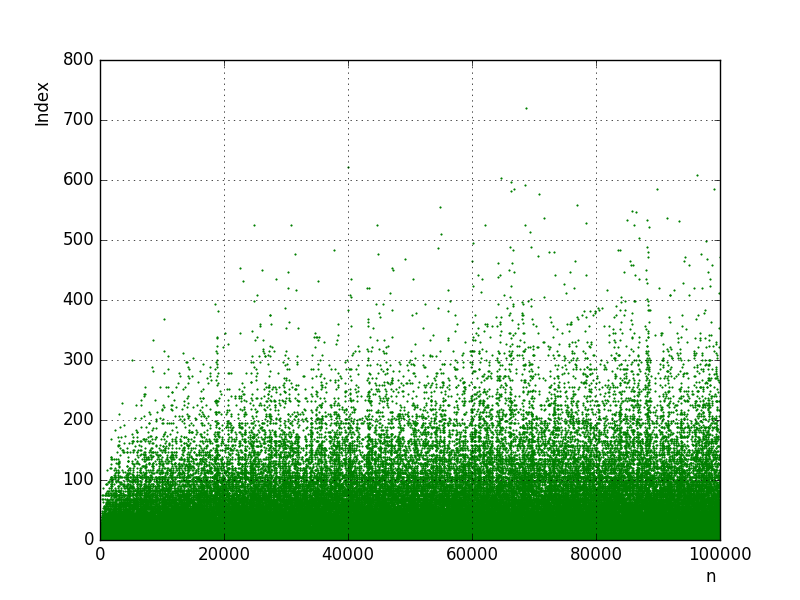
\includegraphics[width=9cm]{f_checkpoint_gap_min_index_sym_primes}
\caption{Minimal $i$ in $psym(n,i)$ ($n$ \textless $10^5$)}
\label{fig:minsymprimeindex}
\end{figure}

\begin{figure}[!ht]
\centering
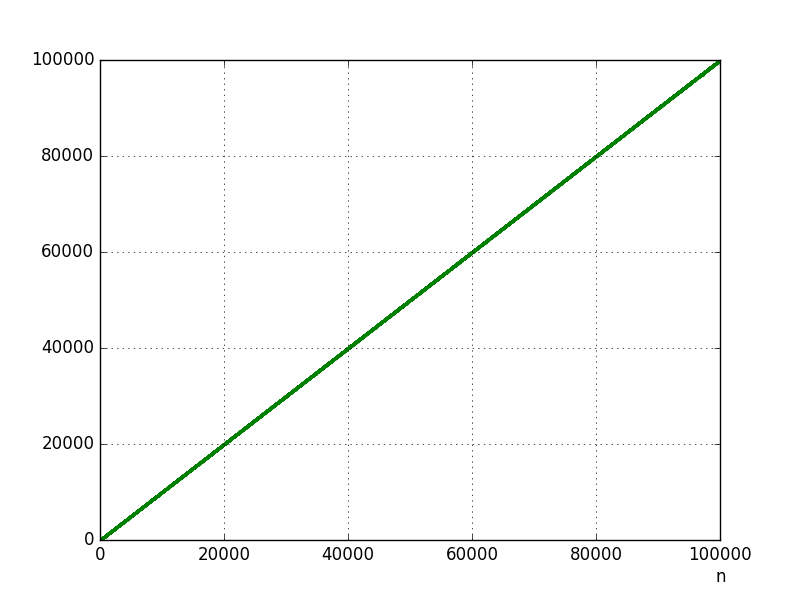
\includegraphics[width=9cm]{f_checkpoint_gap_max_index_sym_primes}
\caption{Maximum $i$ in $psym(n,i)$ ($n$ \textless $10^5$)}
\label{fig:maxsymprimeindex}
\end{figure}

\begin{figure}[!ht]
\centering
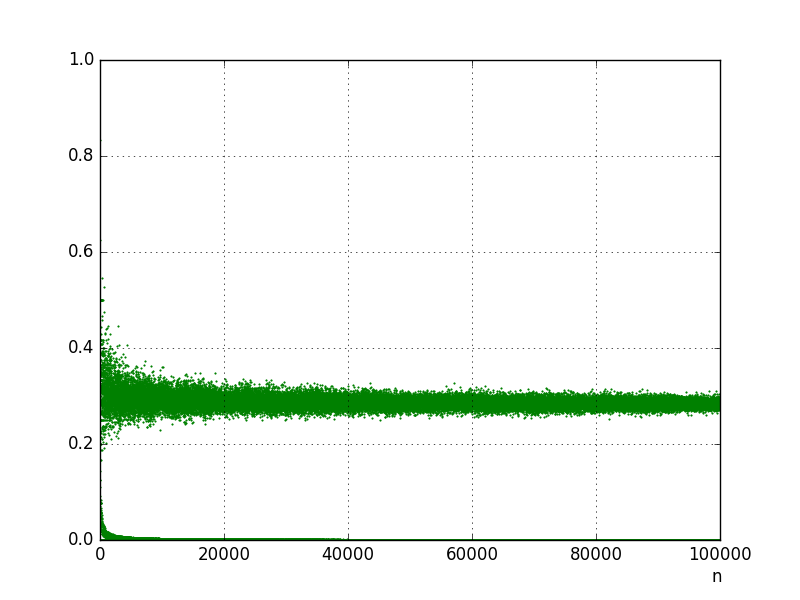
\includegraphics[width=9cm]{f_checkpoint_gap_ratio_to_goldbach}
\caption{$r(n)$ / $s(n)$ ($n$ \textless $10^5$)}
\label{fig:gptosymp}
\end{figure}

\begin{lemma}
If integer $n$ is a half of the sum of two primes then $n$ can be expressed as either $3x - 1$ or $3x$ or $3x + 1$, where $x$ is integer $\geq$ 1.
\end{lemma}
\begin{proof}
Based on Lemma 1, every prime $p$ \textgreater 3 is a form of 6$k$ $\pm$ 1 (where $k \geq 1$). Sum of two primes $s_i$ is then in $3$ variants ($k_i$ is integer $\geq 1$, $k_3 = k_1 + k_2$): $s_1 = 6k_1 - 1 + 6k_2 - 1 = 6k_3 - 2$; $s_2 = 6k_1 - 1 + 6k_2 + 1 = 6k_3$; $s_3 = 6k_1 + 1 + 6k_2 + 1 = 6k_3 + 2$. We will have then: $\frac{s_1}{2} = 3k_3 - 1$; $\frac{s_2}{2} = 3k_3$; $\frac{s_3}{2} = 3k_3 + 1$. Lemma is then true if both primes are \textgreater 3. Let us then analyze all missing cases with primes $\leq 3$: $2$ and $3$. If one of the primes is $2$, then sum of the primes can only be even (so that divided by $2$ gives integer) if second prime is also $2$. This gives us: $\frac{2 + 2}{2} = 2 = 3 \times 1 - 1$, which fulfills the lemma. If one of the primes is $3$, then the second prime cannot be $2$ and can be either $3$ or prime $\textgreater 3$. If second prime is $3$, then we have $\frac{3+3}{2} = 3 = 3 \times 1$, which fullfills the lemma. If second prime is $\textgreater 3$, then we have the following variants: $s_4 = 3 + 6k_2 - 1 = 6k_2 + 2$; $s_5 = 3 + 6k_2 + 1 = 6k_2 + 4 = 6(k_2 + 1) - 2$. We have then: $\frac{s_4}{2} = 3k_2 + 1$;  $\frac{s_5}{2} = 3(k_2 + 1) - 1$, which also fullfills the lemma.
\end{proof}

Every positive integer $n \textgreater 1$ can be expressed as $6a+m$, where $m=0, 1, \ldots, 5$ and $a \geq 0$. Let us analyze all possible solutions in integer numbers if we confront this with Lemma 3 - we will have six (from a) to f)) cases then:

a)
$$
6a = \left\{ \begin{array}{ll}
3x - 1 & \textrm{if $x = 2a + \frac{1}{3}$}\\
3x & \textrm{if $x = 2a$}\\
3x + 1 & \textrm{if $x = 2a - \frac{1}{3}$}
\end{array} \right.
$$

b)
$$
6a + 1 = \left\{ \begin{array}{ll}
3x - 1 & \textrm{if $x = 2a + \frac{2}{3}$}\\
3x & \textrm{if $x = 2a + \frac{1}{3}$}\\
3x + 1 & \textrm{if $x = 2a$}
\end{array} \right.
$$

c)
$$
6a + 2 = \left\{ \begin{array}{ll}
3x - 1 & \textrm{if $x = 2a + 1$}\\
3x & \textrm{if $x = 2a + \frac{2}{3}$}\\
3x + 1 & \textrm{if $x = 2a + \frac{1}{3}$}
\end{array} \right.
$$

d)
$$
6a + 3 = \left\{ \begin{array}{ll}
3x - 1 & \textrm{if $x = 2a + \frac{4}{3}$}\\
3x & \textrm{if $x = 2a + 1$}\\
3x + 1 & \textrm{if $x = 2a + \frac{2}{3}$}
\end{array} \right.
$$

e)
$$
6a + 4 = \left\{ \begin{array}{ll}
3x - 1 & \textrm{if $x = 2a + \frac{5}{3}$}\\
3x & \textrm{if $x = 2a + \frac{4}{3}$}\\
3x + 1 & \textrm{if $x = 2a + 1$}
\end{array} \right.
$$

f)
$$
6a + 5 = \left\{ \begin{array}{ll}
3x - 1 & \textrm{if $x = 2a + 2$}\\
3x & \textrm{if $x = 2a + \frac{5}{3}$}\\
3x + 1 & \textrm{if $x = 2a + \frac{4}{3}$}
\end{array} \right.
$$

In each case just one subcase has solution where both $x$ and $a$ are integers. Table $\ref{tablesymprimes}$ presents these solutions, suplemented by candidates for prime pairs which can produce a given integer symmetry point. Table $\ref{tablesymprimes}$ is taking advantage of Lemma 2 for numbers $\geq 6$ and contains manual calculations for exact symmetrical primes if $2 \leq n \leq 5$. Lemma 2 is also useful when symmetry point $n$ is of form $3x$ and $n \textgreater 3$ - in such case $psym(n,0)$ does not exist because $n$ cannot be prime. Additionaly, $2 \mid k_1 + k_2$ in each row of Table $\ref{tablesymprimes}$, otherwise $\frac{p_1 + p_2}{2}$ would not be integer. If $n=6a$ or $n=6a+3$ ($a \geq 1$) (both numbers are of form $3x$), then $psym(n, n-3)$ does not exist because of Lemma 4.

\begin{lemma}
If $n = 3a$ ($a$ is integer $\textgreater 1$), then $3$ cannot be a symmetric prime to $n$.
\end{lemma}
\begin{proof}
If $p_1 = 3$ is going to be symmetric prime to $n$, then the second prime in symmetry pair is $p_2 = 2n - 3$. If $n = 3a$, then $p_2 = 2 \times 3a - 3 = 3 \times (2a - 1)$. If $2a - 1 \textgreater 1$, then $p_2$ is a composite number (divisors: $3$ and $2a - 1$). $2a - 1$ is always $\textgreater 1$ if $a$ is integer $\textgreater 1$.
\end{proof}

\section{GP confirmation algorithm}

The gist of this work studies various approaches to GP confirmation for consecutive even numbers. First class of methods (Class A) is representing top-down approach which is expressing a given even number $n$ \textgreater 2 as a possible sum of two components $p_1$ and $p_2$ first, and then checks their primality.
Second method class (Class B), a member of bottom-up solutions, is iterating over possible sums built from two numbers $p_1$ and $p_2$, both confirmed as primes in advance. Third method (Class C) is looking for the symmetrical primes $p_1$ and $p_2$ around $n$ \textgreater 1.

\subsection{Class A: primality test of possible components}

Listing 4 depicts algorithm base $A$ used to find the first GP confirmation using primality test of one or two components, $p_1$ and $p_2$, which sum is producing odd number $n$ subjected to GP check. \par
There are two input parameters in the presented approach: starting point for the first round of GP check (initial values of $p_1$ and $p_2$) and next step details to calculate new values of $p_1$ and $p_2$ if the previous interation failed. Starting point could be also expressed as $p_1$/$p_2$ ratio. Next step value could be either constant or variable. As a result algorithm returns GP details (values of $p_1$ and $p_2$, both primes). In addition, in order to compare different versions of algorithms, it returns both number of iterations (denoted as $I(A)$) and total duration of internal calculations. Algorithm throws exception if no GP is found and there is no further iteration possible (next candidate for either $p_1$ or $p_2$ is smaller than the smallest prime 2).\par
It is reasonable to set initial $p_1$ and $p_2$ values as odd numbers (there is just one GP where any of GP factors could be even: 4 = 2 + 2), otherwise first iteration (excluding GP for 4) would always fail. \par
If $p_1$ and $p_2$ are odd, then the next step value (calculated in case of fail) should be a number that will not produce even number as the next candidate for neither $p_1$ nor $p_2$ - it should be a mutliple of 2. There is also a risk that in case of too big next step value algorithm loop would go to the end without finding a candidate in between. Although we are still empirically confirming GP correctness (in other words: there might be even $n$ for which GP is not possible) but if we miss any possible candidate in between going back could be a troublesome. Having that in mind, next step value = 2 looks reasonable - we are moving slowly, one by one through odd numbers - we will not miss any possible prime number. \par
It is also important to mention that all parallel runs take advantage of the same prime and composite number sets. If a given number $p$ exists in either prime set or composite set, primality test gives instant result. This means that only the first run for number $p$ which does not exist in neither prime set nor composite set pays price for full primality test, influencing significantly on time of the processing.\par

\begin{table}[t]
\centering
\caption{Summary of algorithm A variants}
\label{tablealgo}
\begin{tabular}{|c|l|c|}
  \hline 
  \rowcolor{LightCyan}
  Variant & Initial $p_1$ and $p_2$  & Delta \\
  \hline 
  $A_1$ & $p_1$ = $n/2$   & -2 \\
       & $p_2$ = $n$ - $p_1$ & \\
       & if $p_1$ \% 2 == 0:  &\\
       & \hspace{0.2cm} $p_1$ -= 1         & \\
       & \hspace{0.2cm} $p_2$ += 1       & \\
  \hline
  $A_2$ & $p_1$ = 3   & +2 \\
       &  $p_2$ = $n$ - $p_1$  &\\
  \hline 
  $A_3$ & $p_1$ = int($n$/3)  & -2 \\
       & $p_2$ = $n$ - $p_1$ & \\
       & if $p_1$ \% 2 == 0:  &\\
       & \hspace{0.2cm} $p_1$ -= 1         & \\
       & \hspace{0.2cm} $p_2$ += 1       & \\
  \hline
  $A_4$ & $p_1$ = 5   & +2 \\
       &  $p_2$ = $n$ - $p_1$  &\\
  \hline 
  $A_5$ & $p_1$ = 5   & variable \\
       &  $p_2$ = $n$ - $p_1$  & = 0 for iter 0 \\
       &  & = -2 for iter 1 \\
       &  & = +4 for iter 2 \\
       &  & = +2 for iter \textgreater 2 \\
  \hline 
  $A_6$ & $p_1$ = 3   & variable \\
       &  $p_2$ = $n$ - $p_1$  & $p_1$ = next prime \\
  \hline 
  $A_7$ & $p_1$ = 3   & variable \\
       &  $p_2$ = $n$ - $p_1$  & $p_1$ = next twin prime \\
  \hline 
\end{tabular} 
\end{table}

Seven variants of algorithm $A$ are being considered, all based on sieve which is testing primality of each element of a candidate for GP (Table $\ref{tablealgo}$). Variants differ with initial values of $p_1$ + $p_2$ and delta used to calculate next candidates. All variants assume that $p_1 \leq p_2$ and both numbers are always odd (n \textgreater 4 to exclude 4 = 2+2 case). In case of primality test failure for a given pair $p_1$ and $p_2$, the next pair of candidates is changed in regular ($A_1$, $A_2$, $A_3$, $A_4$ - $p_1$ is increased by delta and $p_2$ is decreased by delta) or variable ($A_5$, $A_6$, $A_7$ - delta is a function of iteration) way (Listing 2, Listing 3). Programatically it was possible to keep the same source code for all variants, including $delta()$ (which is a function of iteration) passed to the function as a lambda expression.\par

\lstset{language=Python}
\lstset{breaklines=true}
\lstset{frame=shadowbox}
\lstset{caption={Constant delta}}
\begin{lstlisting}[linewidth=8.7cm]
def delta_constant_plus (i):
  return 2

def delta_constant_minus (i):
  return -2
\end{lstlisting}

The first variant, $A_1$, based on observation depicted in Figure $\ref{fig:mindiff}$, is assuming that difference between primes in GP is small (in comparison to $n$). Initial values of $p_1$ and $p_2$ will be the first matching odd numbers around $\frac{n}{2}$. \par
The second variant, $A_2$, based on observation depicted in Figure $\ref{fig:minprime}$, is assuming that one of the primes in GP is small (in comparison to $n$). $p_1$ starts from 3 but not 2 because $n$ - 2 would never be prime for $n$ \textgreater 4. \par
The third variant, $A_3$, is a proposal in between $A_1$ and $A_2$, with starting point about one third of $n$. \par
The fourth variant, $A_4$, is identical to $A_2$ except starting point: $p_1$ = 5, $p_2$ = n - 5. \par
The fifth variant, $A_5$, is more flexible than $A_4$. $p_1$ also starts from 5 but it checks $p_1$ = 3, and then $p_1$ = 7 and next odd numbers.\par
The sixth variant, $A_6$, is identical to $A_2$ except that next step lenght is variable. $p_1$ is always prime (for $i^{th}$ iteration it is $i^{th}$ prime number). \cite{oliveira2012} calculated that 9781 ($1206^{th}$ prime) is the biggest known prime (so far) required in such approach. $delta\_prime()$ starts from $3$ because all numbers $n$ subjected to Goldbach partitioning are greater than $4$, so they will not have $2$ in their $R(n)$. \par
The seventh variant, $A_7$, is a mutation of $A_6$ - $p_1$ is always a twin prime. $delta\_twinprime()$ starts from $3$ because this is the first twin prime.\par

\lstset{language=Python}
\lstset{breaklines=true}
\lstset{frame=shadowbox}
\lstset{caption={Variable delta}}
\begin{lstlisting}[linewidth=8.7cm]
# input: iteration
# output: delta for next iteration
def delta_variable (i):
  if i == 0:
    delta=0
  elif i == 1:
    delta=2
  elif i == 2:
    delta=-4
  elif i > 2:
    delta=2
  return delta

# input: iteration
# output: delta for next iteration
def delta_prime (i):
  if i == 0:
    delta=0
  else:
    delta=get_ith_prime(i+1)-get_ith_prime(i)
  return delta

# input: iteration
# output: delta for next iteration
def delta_twinprime (i):
  if i == 0:
    delta=0
  else:
    delta=get_ith_twinprime(i)-get_ith_twinprime(i-1)
  return delta

# primes[] = [2, 3, 5, 7 ...]
# twin_primes[] = [3, 5, 7, 11 ...]

# input: index of prime
# output: prime
function get_ith_prime (i):
   return primes[i]

# input: index of twin prime
# output: twin prime
function get_ith_twinprime (i):
   return twin_primes[i]

\end{lstlisting}

\lstset{language=Python}
\lstset{breaklines=true}
\lstset{frame=shadowbox}
\lstset{caption={Fast search algorithm scheme A}}
\begin{lstlisting}[linewidth=8.7cm]
# input: initial p1 and p2 candidates
#    (p1+p2=n)
#    delta - function to calculate
#       next p1 and p2 candidates
# output: final p1 and p2 pair 
#    (both primes, p1+p2=n),
#    time elapsed to find this pair
#    number of iterations required
# exception:
#   when no partition is found
def search_for_partition (p1, p2, delta):
  found=False
  iteration=0
    
  startTime=time.time()
  while not found:
    iteration+=1
    if is_prime(p1) and is_prime(p2):
      found=True
    if not found:
      p1-=delta(iteration)
      p2+=delta(iteration)
    if p1 < 2 or p2 < 2:
      raise ("GPnotFound")
  duration=time.time()-startTime

  return p1, p2, duration, iteration
\end{lstlisting}

\subsection{Class B: sum built from primes}

Listing 5 depicts algorithm base $B$ used to find GP confirmation using two primes sum building approach. \par

\lstset{language=Python}
\lstset{breaklines=true}
\lstset{frame=shadowbox}
\lstset{caption={Fast search algorithm scheme B}}
\begin{lstlisting}[linewidth=8.7cm]
# input: min and max indices of first prime
# external dependencies:
#   S1 - a set of numbers to be verified
#   S2 - a set of numbers already verified
#   N - number below which all even numbers were already verified
#   add_nums() - updates S1
#   remove_nums() - updates S1, S2, N
# output: S1, S2, N
function check_possible_sums (min_ip1, max_ip1):
  for ip1 in range (min_ip1, max_ip1):
    p1 = get_ith_prime(ip1)
    add_nums (2*p1)
    
    for ip2 in range (1, ip1+1):
      p2 = get_ith_prime(ip2)
      num = p1 + p2
      remove_nums  (num, 2*p1)
\end{lstlisting}

In contradiction to $A$ in approach $B$ primality test in direct loop is not required because both components, $p_1$ and $p_2$, are already prime numbers. $B$ is iterating over possible pairs (starting from prime 3, prime number 2 is excluded from calculations because there is only one even number 4 with 2 in its GP) and collects information about possible sums (which are always even because both primes are odd). Let us define an even number $N_{conf}$ below which all even numbers were already confirmed from GP standpoint. It is highly probable that $N_{conf}$ would grow up along with progress of the algorithm because $r(n)$ grows with bigger $n$ (Figure $\ref{fig:pairs}$). There is no point in doing any calculations for any $p_1$ + $p_2$ $\leq$ $N_{conf}$ because this part was already confirmed. Assuming that for a given $p_1$ we iterate down over $p_2$ from $p_1$ to $p_m$ (where $p_1$ + $p_m$ \textgreater $N_{conf}$) the most favourable situation would be if after completing all checks for $p_1$ and $p_2$ we have $N$ = 2 $\times$ $p_1$ - next iteration would not inherit any backlog.

\subsection{Class C: looking for symmetric primes}

Listing 6 presents algorithm base $C$ used to find GP confirmation for even $n$ by finding symmetrical primes to $\frac{n}{2}$. Like in approach $A$, $C$ requires primality test inside the algorithm loop. $C$ has two input parameters: symmetry point and function $delta()$ used to calculate next pair of prime candidates ($p_1$, $p_2$) if both current values are not primes yet. \par

\begin{table}[ht]
\centering
\caption{Summary of algorithm C variants}
\label{tablealgo}
\begin{tabular}{|c|l|c|}
  \hline 
  \rowcolor{LightCyan}
  Variant & Initial value of $i$ & Delta $i$ \\
  \hline 
  $C_1$ & 0 & 1 \\
  \hline
  $C_2$ & 0 & 1 if $n$ is even  \\
  & & 2 if $n$ is odd \\
  \hline 
\end{tabular} 
\end{table}

\lstset{language=Python}
\lstset{breaklines=true}
\lstset{frame=shadowbox}
\lstset{caption={Fast search algorithm scheme C}}
\begin{lstlisting}[linewidth=8.7cm]
# input: n
#    n = (p1 + p2) / 2
#    delta - function to calculate
#       next p1 and p2 candidates
# output: final p1 and p2 pair 
#    (both primes, p1+p2=n),
#    time elapsed to find this pair
#    number of iterations required
# exception:
#   when no symmetrical primes were found
def search_for_sym_primes (n, delta):
  found=False
  iteration=0

  startTime=time.time()
  p1=n
  p2=n
  while not found:
    iteration+=1
    if is_prime(p1) and is_prime(p2):
      found=True
    if not found:
      p1-=delta(iteration)
      p2+=delta(iteration)
    if p2 < 2 or p1 < 2:
      raise Exception ("SymPrNotFound")
  duration=time.time()-startTime

  return p1, p2, duration, iteration
\end{lstlisting}

\section{Results of experiments}

\subsection{Experiments against class A}

All seven variants of class $A$ of GP search algorithm were subjected to programmatic verification against all even numbers 14 \textless $n$ \textless $4  \times 10^8$. Calculations show that $A_2$ required 5 times less iterations than both $A_1$ and $A_3$ (Figure $\ref{fig:alg_iterations}$). Results for $A_2$ and $A_5$ are comparable - number of iterations look almost identical (Figure $\ref{fig:alg_iterations_second}$ - line for $A_2$ covers line for $A_5$) while $A_4$ is worse than $A_2$ and $A_5$. The best results achieved $A_6$. In comparison to $A_2$ (Figure $\ref{fig:alg_iterations_third}$) this approach is using preloaded list of first primes and thanks to that is able to avoid primality checks for $p_1$ ($p_1$ is always prime), algorithm variant does not have to check a case when both candidates are not primes - only primality test of $p_2$ matters. $A_7$ was slightly worse than $A_6$. \par

\begin{figure}[!ht]
\centering
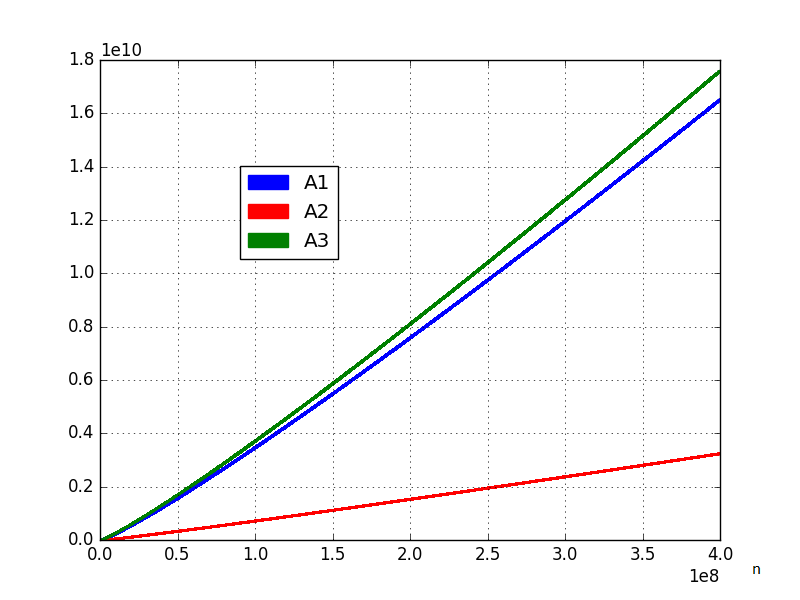
\includegraphics[width=9cm]{f_checkpoint_iters_alg}
\caption{Iterations - $A_1$ vs $A_2$ vs $A_3$ ($n$ \textless $4  \times 10^8$), $A_2$ is the best one: I($A_3$) \textgreater I($A_1$) \textgreater I($A_2$)}
\label{fig:alg_iterations}
\end{figure}

\begin{figure}[!ht]
\centering
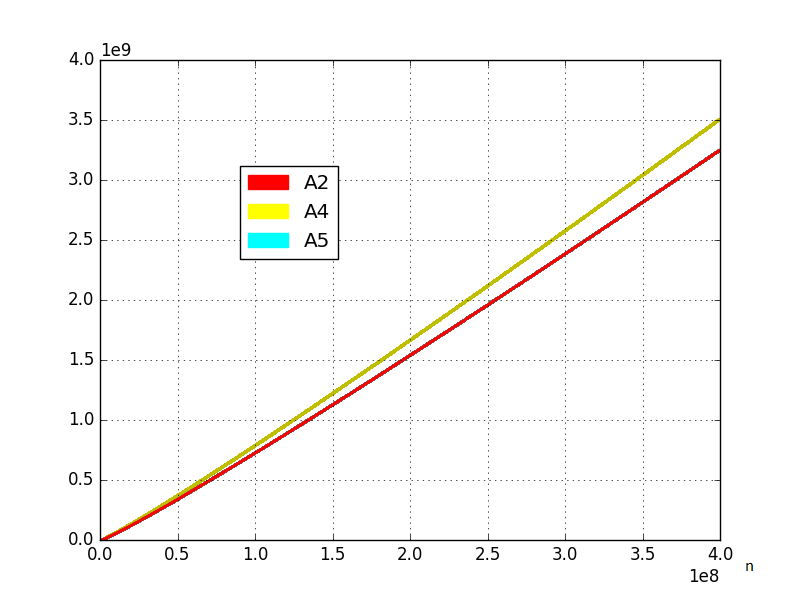
\includegraphics[width=9cm]{f_checkpoint_iters_alg_second}
\caption{Iterations - $A_2$ vs $A_4$ vs $A_5$ ($n$ \textless $4  \times 10^8$), $A_2$ is the best one: I($A_4$) \textgreater I($A_5$) $\geq$ I($A_2$)}
\label{fig:alg_iterations_second}
\end{figure}

\begin{figure}[!ht]
\centering
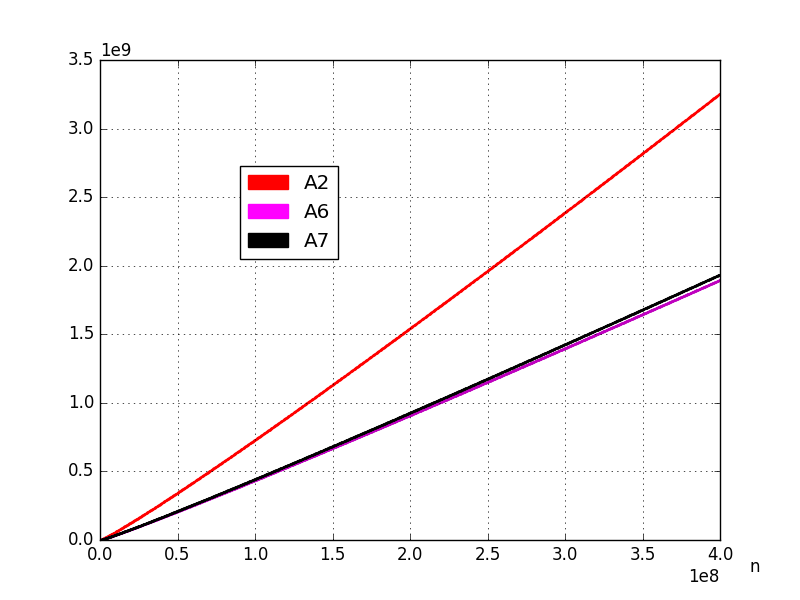
\includegraphics[width=9cm]{f_checkpoint_iters_alg_third}
\caption{Iterations - $A_2$ vs $A_6$ vs $A_7$ ($n$ \textless $4  \times 10^8$), $A_6$ is the best one: I($A_2$) \textgreater I($A_7$) \textgreater I($A_6$)}
\label{fig:alg_iterations_third}
\end{figure}

Results achieved by $A_6$ suggest that properties depicted by Figure $\ref{fig:maxdiff}$ and Figure $\ref{fig:minprime}$ are strong and still preserved for $n$ \textgreater $10^6$. Assuming that efficiency of primality test can be improved, $A_6$ looks like the best choice amongst all examined $A$s. $A_6$ requires prework - a list of first primes for $p_1$ - but such preloaded set is not a big issue for modern computers and may be reused in primality test.

\subsection{Experiments against class B}

Effectiveness of sum building from prime numbers is very high. Each round of algorithm $B$ has a theoretical maximum even number $N_{max}$ below which all numbers are already verified: $N_{max} = max(p_1, p_2) \times 2$. Detailed examination of difference between $N_{max}$ and $N_{conf}$ show that this difference is low: both lines in Figure $\ref{fig:sum_build_effectiveness}$ almost match (although $N_{max} = N_{conf}$ for iterations $0$, $1$, $2$, $4$, $6$ and $27$ only, for other cases calculated so far $N_{max} \textgreater N_{conf}$), red values in Figure $\ref{fig:sum_build_diff}$ are relatively low. Cardinalities of two supporting sets, a set of number to be verified \textgreater $N_{conf}$ and a set of spare verified numbers \textgreater $N_{conf}$, are also low (Figure $\ref{fig:sum_build_spare_and_to_be_verified}$). \par

\begin{figure}[!ht]
\centering
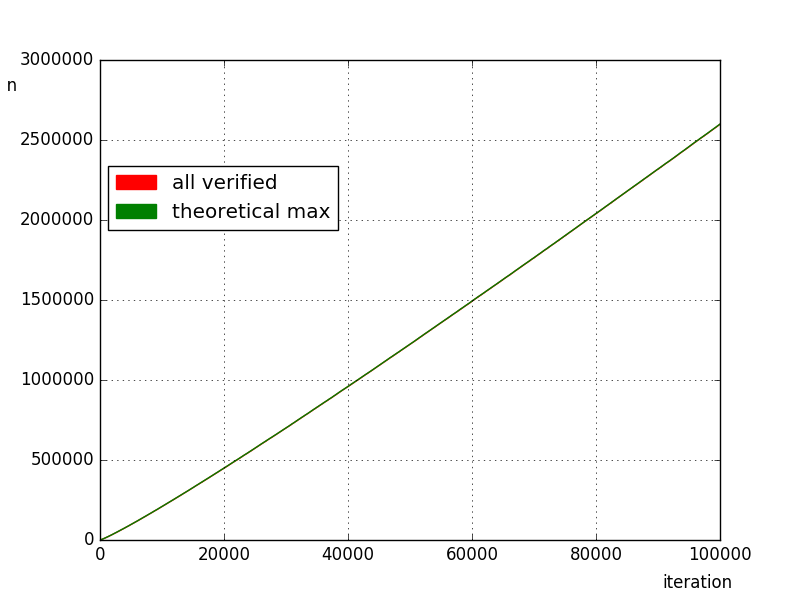
\includegraphics[width=9cm]{f_sum_build_effectiveness}
\caption{Effectiveness of sum building in $B$}
\label{fig:sum_build_effectiveness}
\end{figure}

\begin{figure}[!ht]
\centering
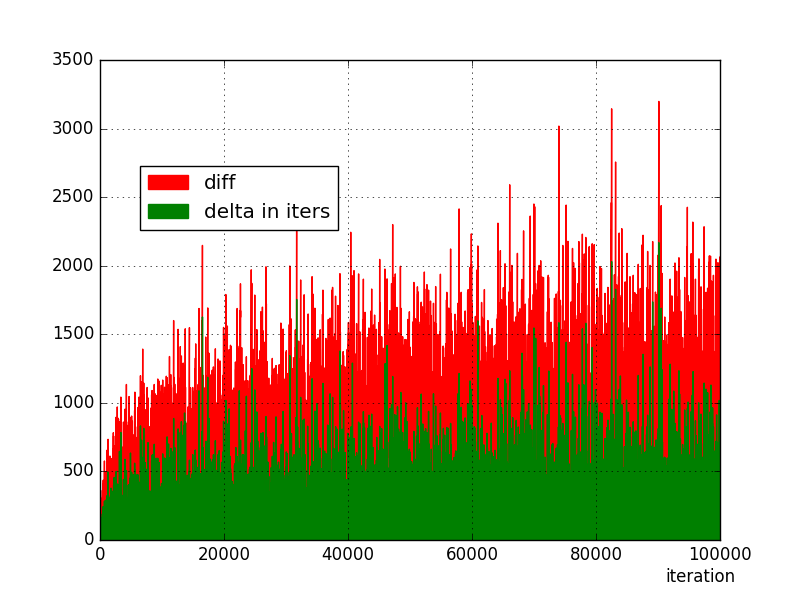
\includegraphics[width=9cm]{f_sum_build_diff}
\caption{Differences in $B$: difference between actual $N_{conf}$ and theoretical maximum $N_{max}$ (in red); absolute difference of red values between individual iterations (in green)}
\label{fig:sum_build_diff}
\end{figure}

\begin{figure}[!ht]
\centering
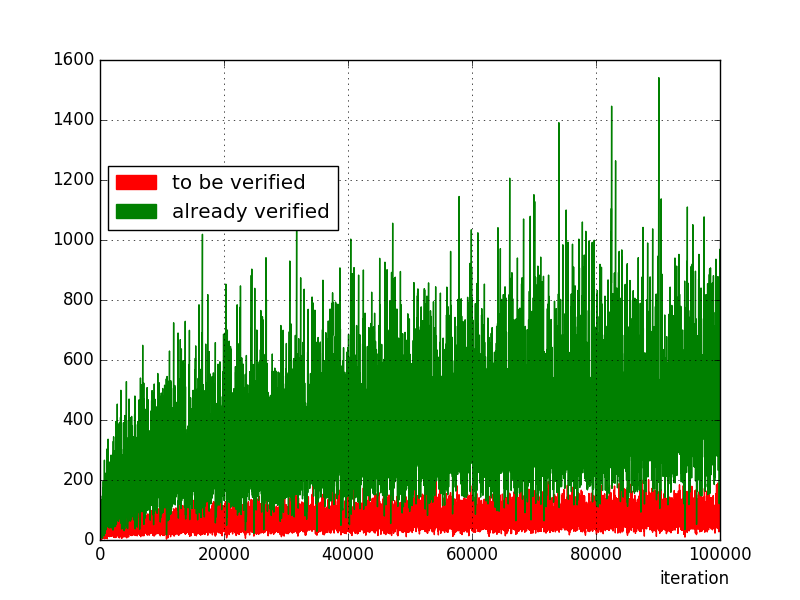
\includegraphics[width=9cm]{f_sum_build_spare_and_to_be_verified}
\caption{Cardinality of two supporting sets in $B$: numbers to be verified \textgreater $N_{conf}$ (in red) and spare numbers already verified \textgreater $N_{conf}$ (in green)}
\label{fig:sum_build_spare_and_to_be_verified}
\end{figure}

\subsection{Experiments against class C}

Executed experiments show that the most effective algorithm in class C is $C_2$.

\begin{figure}[!ht]
\centering
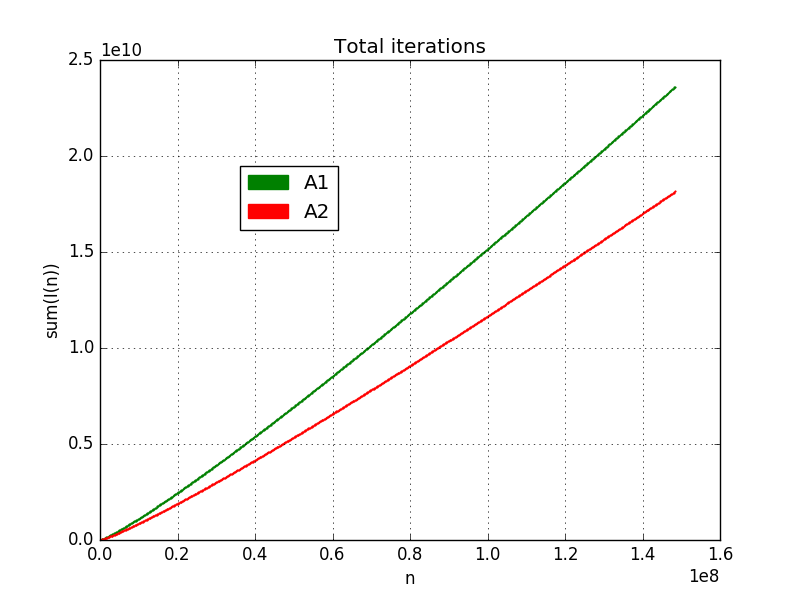
\includegraphics[width=9cm]{f_checkpoint_sym_primes_alg1}
\caption{Iterations - $C_1$ vs $C_2$ ($n$ \textless $4  \times 10^8$), $C_2$ is the best one: I($C_1$) \textgreater I($C_2$)}
\label{fig:sym_primes_alg1}
\end{figure}

\section{Summary and future work}

From all examined algorithm variants of search for the first pair of primes $(p_1, p_2)$ for even $n$ that $GSC(n, p_1, p_2)$ the most promissing results were achieved by $A_6$. When taking into account finding such partition for all consecutive even numbers $n_1, n_2, \ldots n_m$ $A_6$ allowed to find this partition with the least number of iterations. Listing 7 presents skew of distributed version of $A_6$-like approach - initial data range is divided into subintervals and each subinterval is verified independently on a separate compute node. \par

\lstset{language=Python}
\lstset{breaklines=true}
\lstset{frame=shadowbox}
\lstset{caption={Distributed fast search}}
\begin{lstlisting}[linewidth=8.5cm]
def verify (chunk):
   for n in chunk:
      p1 = 3
      p2 = n - 3
      (p1, p2, d, i) = search_for_partition (p1, p2, lambda i: delta_prime(i))

# main
chunks = divide (max, max_chunk_size)
for chunk in chunks:
   verify (chunk)

\end{lstlisting}

Furthermore, studies on GP fast confirmation methods resulted in additional interesting research areas and questions which could be a foundation of further research work. \par
First area relates to frequency of primes in GPs. 2 is the prime number that exists in one GP only ($4 = 2 + 2$) - let's call such prime a selfish prime - and no other prime of such property exists. But how about other most and least frequent primes? Is there any pattern? \par
Second research field may concentrate on finding further mathematical patterns of regular properties observed during above studies. Examples are: bottom and upper estimations of maximum and average difference between primes in GP. 

\begin{thebibliography}{9}

\bibitem{goldbach1742}
  Christian Goldbach, 
  \emph{On the margin of a letter to Leonard Euler},
  1742.
\bibitem{oliveira2012}
  Tomás Oliveira e Silva,
  \emph{Goldbach conjecture verification.}
  http://sweet.ua.pt/tos/goldbach.html,
  2012.
\bibitem{woon2000}
  Max S.C. Woon,
  \emph{On Partitions of Goldbach's Conjecture}, arXiv:math/0010027 [math.GM], 2000.  
\bibitem{github}
  Marcin Barylski,
  \emph{Goldbach conjecture verification framework.}
  https://github.com/mbarylsk/goldbach-partition,
  2016.
\bibitem{barylski2018}
  Marcin Barylski,
   \emph{Studies on Twin Primes in Goldbach Partitions of Even Numbers}, 2018.
\bibitem{barylski2018-2}
  Marcin Barylski,
   \emph{Goldbach Strong Conjecture Verification Using Prime Numbers}, 2018.
\bibitem{oliveira2002}
  Tomás Oliveira e Silva,
  \emph{Fast implementation of the segmented sieve of Eratosthenes.}
  http://sweet.ua.pt/tos/software/prime\_sieve.html,
  2002.
\end{thebibliography}

\end{document}
